

\setcounter{section}{2}
\section{System Components}
\bigskip

\subsection{MCU - ESP32}
\medskip
ESP32 is a series of low-cost, low-power system on a chip microcontrollers with integrated Wi-Fi and dual-mode Bluetooth. Created and developed by Espressif, the ESP32 contains a Tensilica Xtensa LX6 microprocessor in both dual-core and single-core variations and includes a in-built antenna, power amplifier, low-noise receive amplifier, filters, and power-management modules (As shown in figure \ref{esp_core}) \cite{R3-1-1}. 

\medskip
\begin{figure}[H]
\centering
    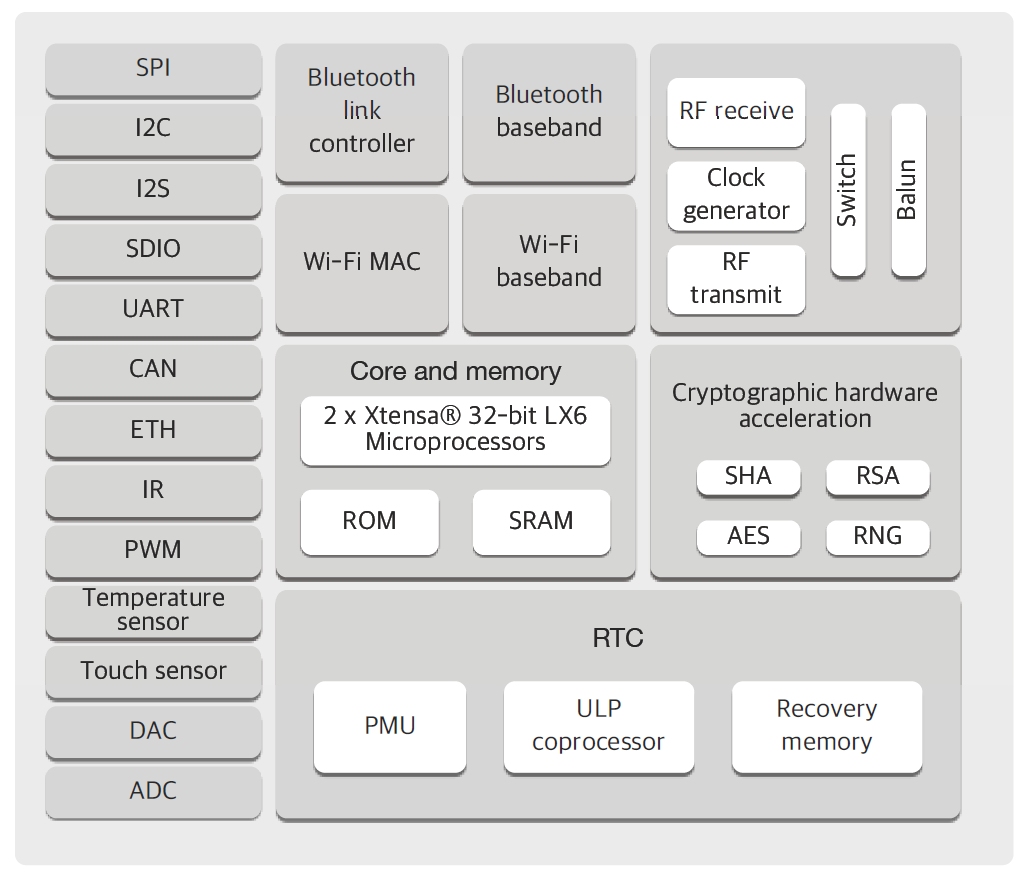
\includegraphics[scale=0.4]{./images/esp_core.png}
    \caption{ESP32 Architect Block Diagram}
    \label{esp_core}
\end{figure}

For the proof of concept, the Bluetooth modules on the ESP32 will be used as the communication interface between the Beacon and the ID tags. Using BLE advertising, the ID Tags ESP32 broadcasts a unique MAC address. The Beacon ESP32 can collect all assicating ID Tag ESP32s and capture the RSSI and MAC of these devices. These information are forwarded to the DPU for distances estimation and location plotting.

\begin{figure}[H]
\centering
    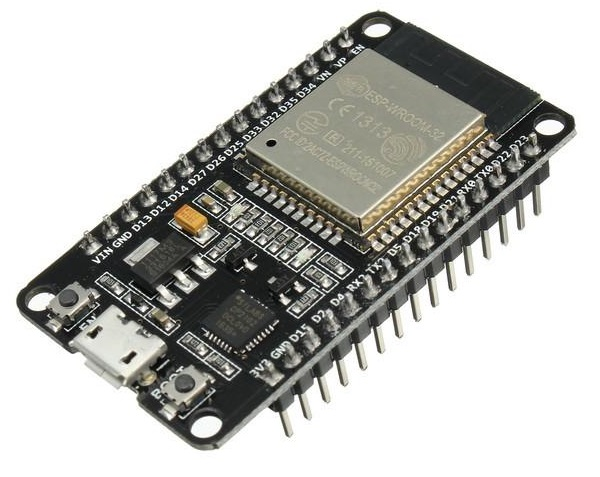
\includegraphics[scale=0.25]{./images/esp.jpg}
    \caption{ESP32 Development Board}
    \label{esp}
\end{figure}


\pagebreak
In the Final design both the Beacon and ID tags will use the ESP32 as the main controller unit but they will be also be incorporated with Decawave DWM1000 UWB modules as the transceivers. The ESP32’s Serial Peripheral Interface (SPI) will be used to interact with the Decawave DWM1000 UWB modules for sending and receiving data. A mock-up circuit diagram presenting the SPI interface between the ESP32 and a breakout board for DWM1000 is shown in figure \ref{eps_dwm_circuit}. In addition, the ESP32 features a deep sleep mode which reduces power consumption to about 10uA from 260mA (active operations), thus drastically increasing the battery life time which is an important constraint for the portable ID tags. In the event of an emergency, the ESP32 can be woken from deep sleep to start transmission by activating a touch pin (\Gls{GPIO} 26-23 shown in Figure \ref{esp_pin}). Furthermore, by utilizing the ESP32's wide range of capabilities such as WiFi or Bluetooth, a mesh network and be implemented to extend the communication range of the Beacons. 

\medskip
\begin{figure}[H]
\centering
    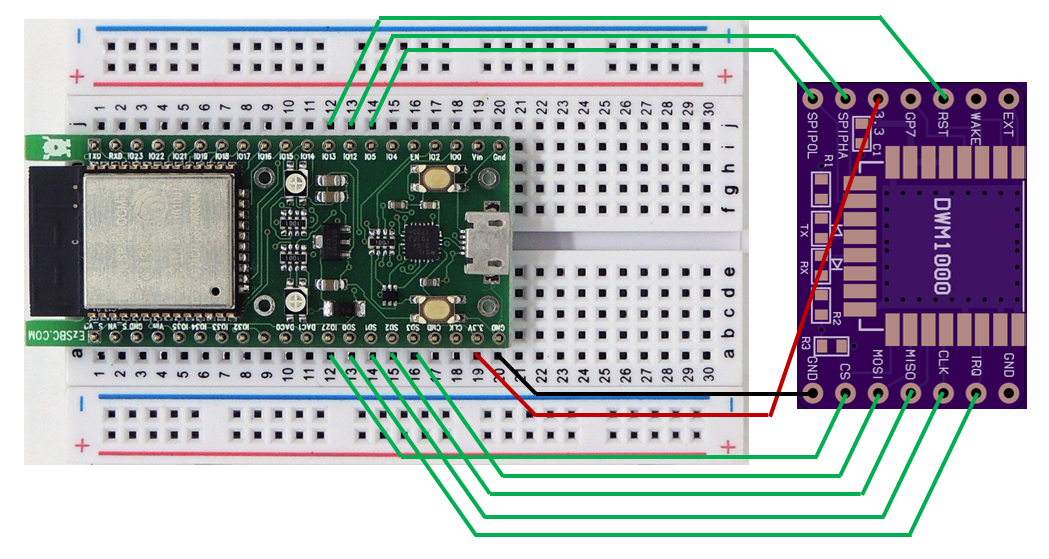
\includegraphics[scale=0.5]{./images/eps_dwm_circuit.png}
    \caption{Circuit Diagram of ESP32 \& DWM1000}
    \label{eps_dwm_circuit}
\end{figure}

\medskip
\begin{figure}[H]
\centering
    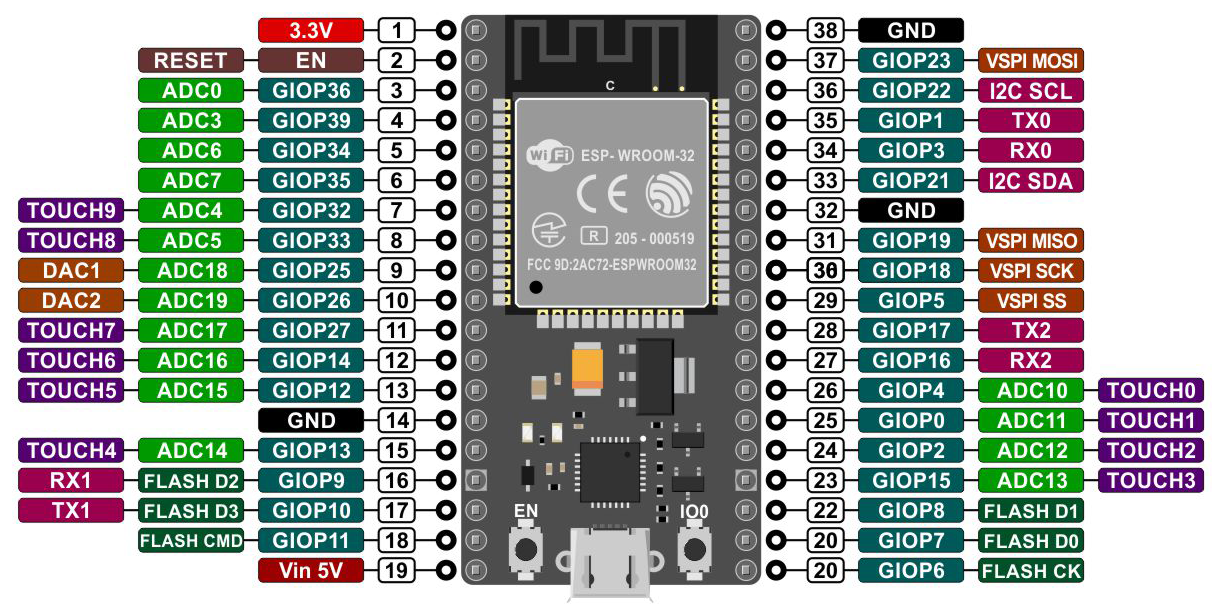
\includegraphics[scale=0.5]{./images/esp32_pin.png}
    \caption{ESP32 Pin Layout}
    \label{esp_pin}
\end{figure}


\pagebreak
\subsection{Transceiver - DWM1000} 
\medskip
The Beacon and ID Tag communication will be done using ultra-wideband wireless communication in the prototype phase and beyond. The most optimal transceiver available on the market that best fits the needs and scope of this project is the Decawave DWM1000 UWB module (Figure \ref{dwm1000}). The DWM1000 is an IEEE 802.15.4-2011 UWB compliant and \Gls{FCC}/\Gls{ETSI} certified wireless transceiver module based on Decawave’s DW1000 IC \cite{R4-2-1}. This module is a combination of DW1000 IC, a built in antenna, power management system, and clock control which allows for simple integrations into any system (Figure \ref{dwm1000_bd}). 

\medskip
\begin{figure}[H]
\centering
    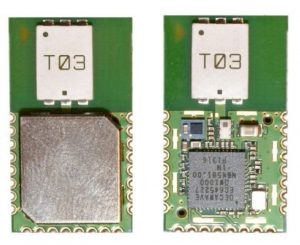
\includegraphics[scale=0.75]{./images/dwm1000.jpg}
    \caption{Decawave DWM1000 Modules}
    \label{dwm1000}
\end{figure}

The module enables the location tracking of objects in real time location systems (RTLS) down to a precision of 10 cm indoors. It supports high range of communications data rates from 110 Kbps to 6.8 Mbps, with excellent communication ranges of up to 300m. The frequencies of operation in the range of 3.5 to 6.5GHz with seven distinct channels which would significantly reduce issues of signal interference or multipath propagation. Its small physical size allows the module to be implemented in highly cost-effective solutions. By using this module, integration with the Akriveia Beacon system is intuitive and simple; since the DWM1000 also offers a wide range of MCU support such as Arduino MCUs or the ESP32 MCUs. 

\medskip
\begin{figure}[H]
\centering
    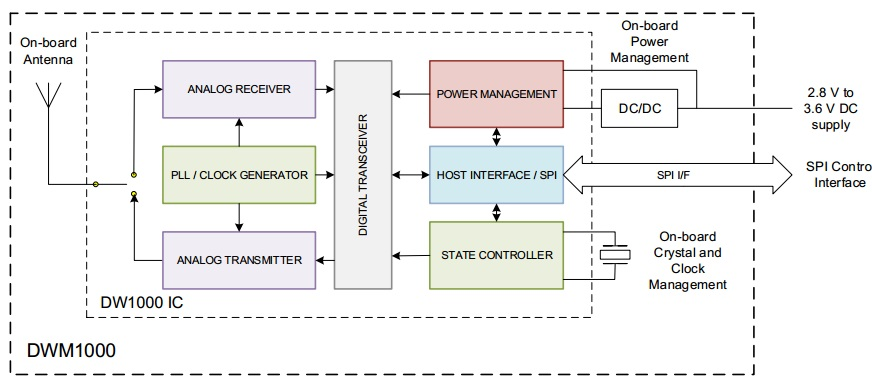
\includegraphics[scale=0.7]{./images/dwm1000_bd.jpg}
    \caption{DWM1000 Internal Block Diagram}
    \label{dwm1000_bd}
\end{figure}



\pagebreak
\subsection{DPU - Raspberry Pi}
\medskip
The Data Processing Unit is a stand alone single board computer (SBC). For the demonstration of this project a Raspberry Pi 3 B+ is used as the DPU since it is an affordable and robust SBC, but the DPU in theory should be any electrical computer device that is capable of running a basic linux operating system; as the software stack is designed to operate on any linux based system. The Raspberry Pi product is cheap, portable and designed with an Cortex-A53 processor it meets the minimum requirements for the DPU.

\bigskip
The Raspberry Pi 3 B+ is a single board computer with a 1.4GHz 64-bit quad-core processor, dual-band wireless LAN, and Bluetooth 4.2/BLE \cite{R3-3-1}. The Broadcom BCM2837B0, Cortex-A53 (ARMv8) 64-bit SoC at 1.4GHz quad-core processor allows complex tri or multilateration calculations done simultaneously for multiple ID Tags. With dual-band 2.4G and 5G IEEE 802.11.b/g/n/ac wireless LAN, the Pi can create a reliable network access for multiple ESP32 for data forwarding. At a power rating of 5V/2.5A \Gls{DC} the Pi requires minimal power to operate, which allows for a variety of power options during emergency disasters. Furthermore, the Pi is configurable with any linux based OS, such as Debian OS which is compatible with the software stack developed in Rust that will create a layer of user interface between the user and the Akriveia Beacon system.


\medskip
\begin{figure}[H]
\centering
    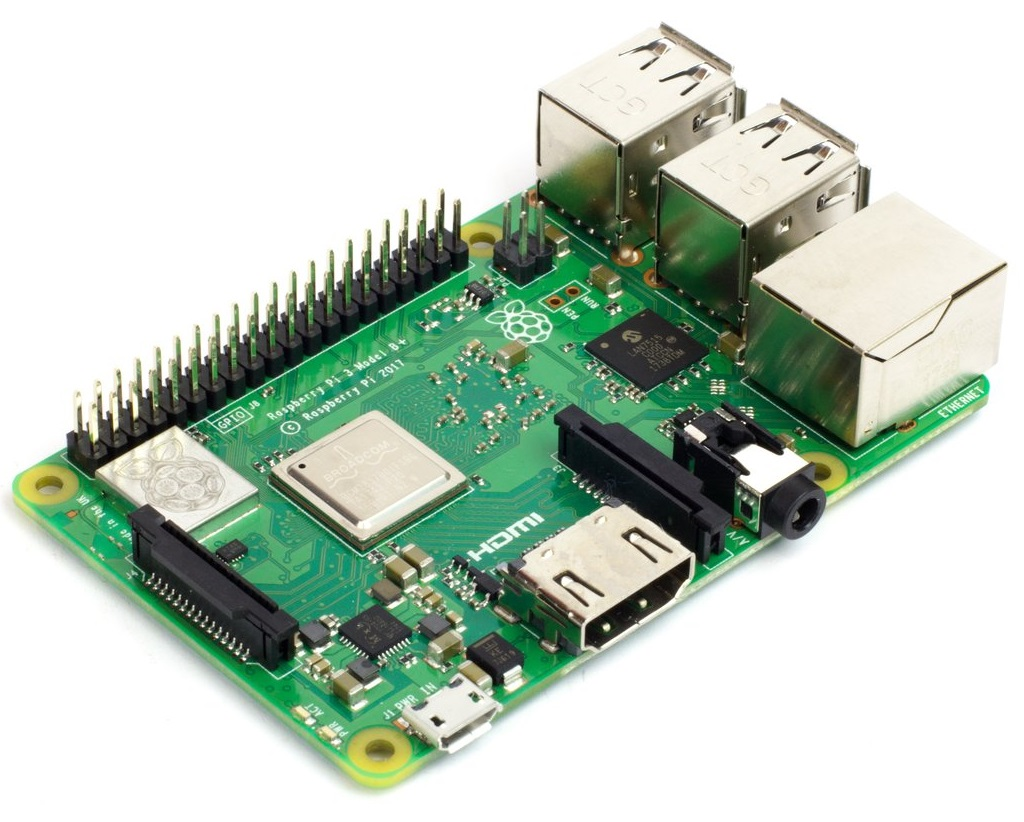
\includegraphics[scale=1]{./images/pi.jpg}
    \caption{Raspberry Pi 3 B+ Model}
    \label{pi}
\end{figure}




